\section{Mechanism: what we found and what we did not}
\label{sec:mechanism}

This section reports observations and conjectures about \emph{how} the learned probability-flow ODE breaks, mostly for $P=I$.
None of it is a claim of the paper.
We use the twelve broken runs of networks 1--4, 7 and 8 with $P=I$ (both seeds).
Their final outliers number 123.
For comparison we follow 200 \emph{tail} points (Mahalanobis distance 3.5--5 to the nearest component of the prior) and 200 \emph{bulk} points (distance below 2) per run that did not become outliers.
The ODE moves every point independently, so a single trajectory can be re-run with a different score on any stretch of the reverse time.

\subsection{Where the breaking trajectories start}

\begin{observation}[tail starts]
\label{obs:tail}
Every final outlier starts in the tail of the prior: their Mahalanobis distances lie between 3.71 and 5.16, while 99\% of all prior points lie below 3.61.
\end{observation}

\subsection{Which stretch of the learned score is needed}

We first replaced the learned score by the exact one on parts of the reverse time (eight runs, networks 1--4).

\begin{test}[H3: the last stretch alone]
\label{test:h3}
Prediction: the break is made by the learned score below $\sigma=0.01$, where the reverse flow locally expands.
(a)~Exact score below $0.01$ removes it in at least 7 of 8 runs; (b)~learned score only below $0.01$ keeps it in at least 5 of 8.
\emph{Both not supported:} (a)~2 of 8; (b)~0 of 8.
With the learned score only below $\sigma_c=0.03$, $0.01$, $0.007$ or $0.006$, no run broke.
With the learned score only above $\sigma_c$, 2, 6, 7 and 8 of the 8 runs broke.
\end{test}

The last stretch is thus harmless when it starts from the right place, and the learned score above $\sigma=0.03$ is necessary.
We then searched for the smallest window of $\sigma$ in which the learned score is needed.
The reverse time was split into eight bands at $\sigma=40$, 1, 0.3, 0.1, 0.05, 0.03, 0.02, 0.01, 0.005, and the learned score was used inside a window of adjacent bands and the exact score outside (36 windows, twelve runs).

\begin{test}[H5: a narrow seed window]
\label{test:h5}
Prediction: a window inside $\sigma\in[0.03,0.1]$ reproduces the break in at least 9 of 12 runs (H5).
Alternative prediction: $[0.01,0.1]$ reproduces it in at least 9, and $[0.03,0.1]$ in at most 3 (H5$'$).
\emph{Both not supported:} no window inside $[0.005,0.1]$ reproduced the break in any run.
In these windows the runs kept no outlier and $|L|\leq0.026$.
\end{test}

\begin{observation}[wide windows]
\label{obs:windows}
Only the full range reproduced the break in all twelve runs [Fig.~\ref{fig:mech}(a)].
The window $[0.01,40]$ reproduced it in 10, and $[0.05,40]$, $[0.03,40]$, $[0.02,40]$ in 6 each.
Windows that exclude $\sigma>1$ reproduced it at most in 5 runs ($[0.005,1]$).
The minimal windows differ between networks: for network 3 the window $[0.3,40]$ suffices, for networks 1 and 4 nearly the full range is needed.
\end{observation}

\subsection{How the deviation grows}

\begin{observation}[deviation before the jump]
\label{obs:deviation}
At $\sigma=0.1$, the final outliers already differ from their exact-score paths by $0.09$--$0.26$ (median per run), against $0.03$--$0.04$ for tail points and $0.005$--$0.007$ for bulk points [Fig.~\ref{fig:mech}(b)].
All deviations shrink until $\sigma=0.01$; in the last band the outliers jump.
\end{observation}

\begin{observation}[the deviation is made early]
\label{obs:bands}
Starting each band on the exact path and using the learned score only inside it, the deviation made within the first band ($\sigma$ from 40 to 1, 1845 of the 4496 steps) has a median of $0.73$ for the outliers, $0.22$ for tail points and $0.04$ for bulk points (medians over the twelve runs).
In every later band it is at most $0.07$ for the outliers.
As a score for telling final outliers from tail points within a run, the deviation made in the first band gives a pooled area under the ROC curve of $0.96$, the prior Mahalanobis distance $0.93$, and the mean score error on the exact path $0.86$.
These areas are in-sample.
For tail points in the other metrics (networks 1--4), the first-band deviation is $0.15$--$0.19$, against $0.20$--$0.23$ for $P=I$.
\end{observation}

\subsection{Exact-score amplification}

If the metric decided the break through the flow alone, a fixed perturbation would be amplified most where breaks are common.
We added the measured learned-minus-exact deviations of the outliers (their sizes and directions, from all twelve runs) to tail points on the exact path at $\sigma_{\rm inj}$, and carried them to the end with the \emph{exact} score.
The amplification is $A=|\Delta x_{\rm end}|/|\Delta z_{\rm inj}|$, with $\Delta x_{\rm end}$ the final position difference to the unperturbed path.

\begin{test}[H6: amplification ordered by $\kP$]
\label{test:h6}
Prediction: at $\sigma_{\rm inj}=0.03$ the median $A$ over tail points is largest for $P=I$ (H6a) and ordered $P=I>\max(\dtwo,\optc{1.25})$, $\min(\dtwo,\optc{1.25})>\optc{5}$ (H6b).
\emph{Both not supported:} $A=6.8$ ($P=I$), $10.5$ ($\dtwo$), $6.6$ ($\optc{1.25}$) and $15.9$ ($\optc{5}$).
The ordering is nearly the reverse, and it is the same at $\sigma_{\rm inj}=0.3$, $0.1$ and $0.01$.
\end{test}

With the exact score, only 2--6\% of the perturbed tail points end as outliers after an injection at $\sigma=0.03$.
The exact-score flow alone does not produce the jump.

\subsection{Learned-score amplification (H9)}
\label{sec:h9}

The remaining candidate for the jump is the learned score itself in the last stretch, where it is evaluated far from the data it was trained on.
We repeated the injection at $\sigma_{\rm inj}=0.01$ with the same perturbations, carrying them to the end (i)~with the exact score and (ii)~with the learned score, for networks 1--4 of every metric.
In (ii) the reference is the unperturbed path under the same learned score, so $A$ measures how much the learned flow itself spreads the perturbation.
The ratio $R=\mathrm{median}\,A_{\rm learned}/\mathrm{median}\,A_{\rm exact}$ is computed per network.

\begin{test}[H9: the jump is an extrapolation of the learned score]
\label{test:h9}
Predictions: (a)~$R\geq10$ for at least 12 of 16 networks; (b)~$R$ is larger for $P=I$ and $\dtwo$ than for $\optc{1.25}$ and $\optc{5}$ (one-sided Mann--Whitney, $p\leq0.05$); (c)~the same ratio of the 90th percentiles, $R_{90}\geq10$, for at least 12 of 16 networks.
(a)~\emph{Not supported:} $R=2.8$--$7.8$, for none of the 16.
(b)~\emph{Not supported:} $p=0.12$; the medians of $R$ are 3.8 ($P=I$), 3.9 ($\dtwo$), 3.4 ($\optc{1.25}$) and 4.1 ($\optc{5}$).
(c)~\emph{Supported:} $R_{90}\geq12$ for all 16 networks, and above $10^4$ for 10 of them.
\end{test}

\begin{observation}[the learned flow amplifies a part of the tail]
\label{obs:h9}
For a typical perturbed tail point the learned flow spreads the perturbation a few times more than the exact flow.
For 19--45\% of them it spreads it at least ten times more, and for the top decile by many orders of magnitude, often to non-finite values.
This holds in every metric, including $\optc{1.25}$, whose networks never broke.
Without a perturbation, the learned flow from the exact state at $\sigma=0.01$ leaves at most 3 of the 291 tail points as outliers.
\end{observation}

\begin{conjecture}
\label{conj:twostage}
The break has two stages.
In the first, the learned score moves a few tail trajectories away from their exact paths, mostly while $\sigma$ is large.
In the second, the learned score in the last stretch, evaluated off the data, amplifies such deviations by orders of magnitude.
The second stage is present in every metric we tested (Test~\ref{test:h9}c), so the metric acts mainly through the first stage, or through the interplay of the two, which the present measurements do not resolve.
\end{conjecture}

The first-stage deviation of tail points is only 1.2--1.5 times larger for $P=I$ than in the other metrics (Observation~\ref{obs:bands}).
Whether this is enough to explain 10 of 12 against 3 of 16 is open.
Two further possibilities are not resolved by our measurements.
The perturbations injected in Test~\ref{test:h9} were collected from the outliers of $P=I$ and added with the same size and direction in every metric, so the test does not probe whether the first-stage deviation differs between metrics in its \emph{direction} as well as in its size.
And since the learned-score amplification is a few-fold for a typical tail point but orders of magnitude for the top decile, a modest change in the first-stage deviation may move a few tail points across a steep threshold.

\subsection{Predicting which network breaks}

\begin{test}[H7: tail score error]
\label{test:h7}
The mean-square score error on tail points over $\sigma\in[0.05,40]$, $e^\ast$, was used with a threshold fitted on networks 1--8 with $P=I$ (7 of 8 correct).
The prediction for four new networks was written and hashed before they were sampled.
\emph{Outcome: 4 of 4 correct, but uninformative:} the rule predicted ``broken'' for all four, as would the base rate (6 of 8 had broken so far).
Across all 24 earlier networks, a single threshold on $e^\ast$ classified only 15 correctly, with the opposite direction.
\end{test}

\begin{figure*}[t]
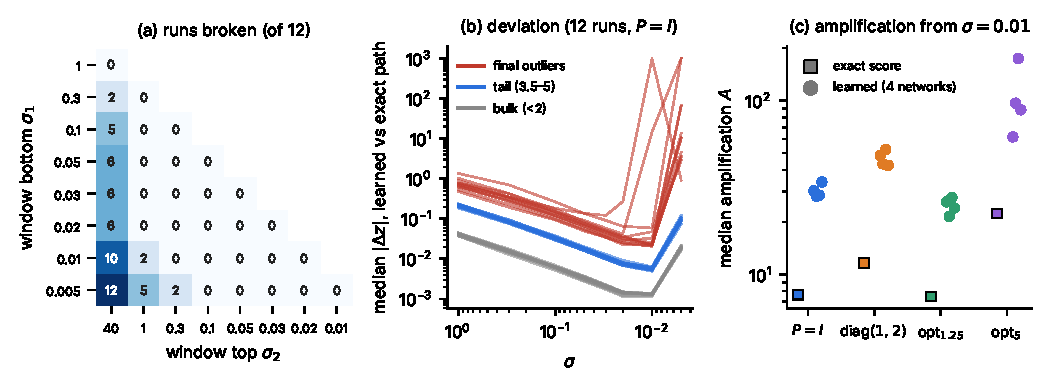
\includegraphics[width=\textwidth]{figures/fig3_mechanism}
\caption{Mechanism, $P=I$ unless stated.
(a)~Number of the twelve broken runs that break again when the learned score is used only in the window $[\sigma_1,\sigma_2]$ and the exact score outside.
(b)~Median deviation between the learned-score and exact-score paths, for the final outliers, tail points and bulk points of each run.
(c)~Median amplification of a measured deviation injected at $\sigma=0.01$ into tail points, carried to the end with the exact score (squares; one value per metric) and with the learned score of networks 1--4 (dots).}
\label{fig:mech}
\end{figure*}
